\section{Experimental Setup}
The setup as drawn in the instructions is shown in \cref{setup1}. In addition to this an actual experimental setup is shown in \cref{setup2}. 
The light source For the beamsize we used a collimating slit of five variable widths.

\begin{figure}[h]
    \centering
    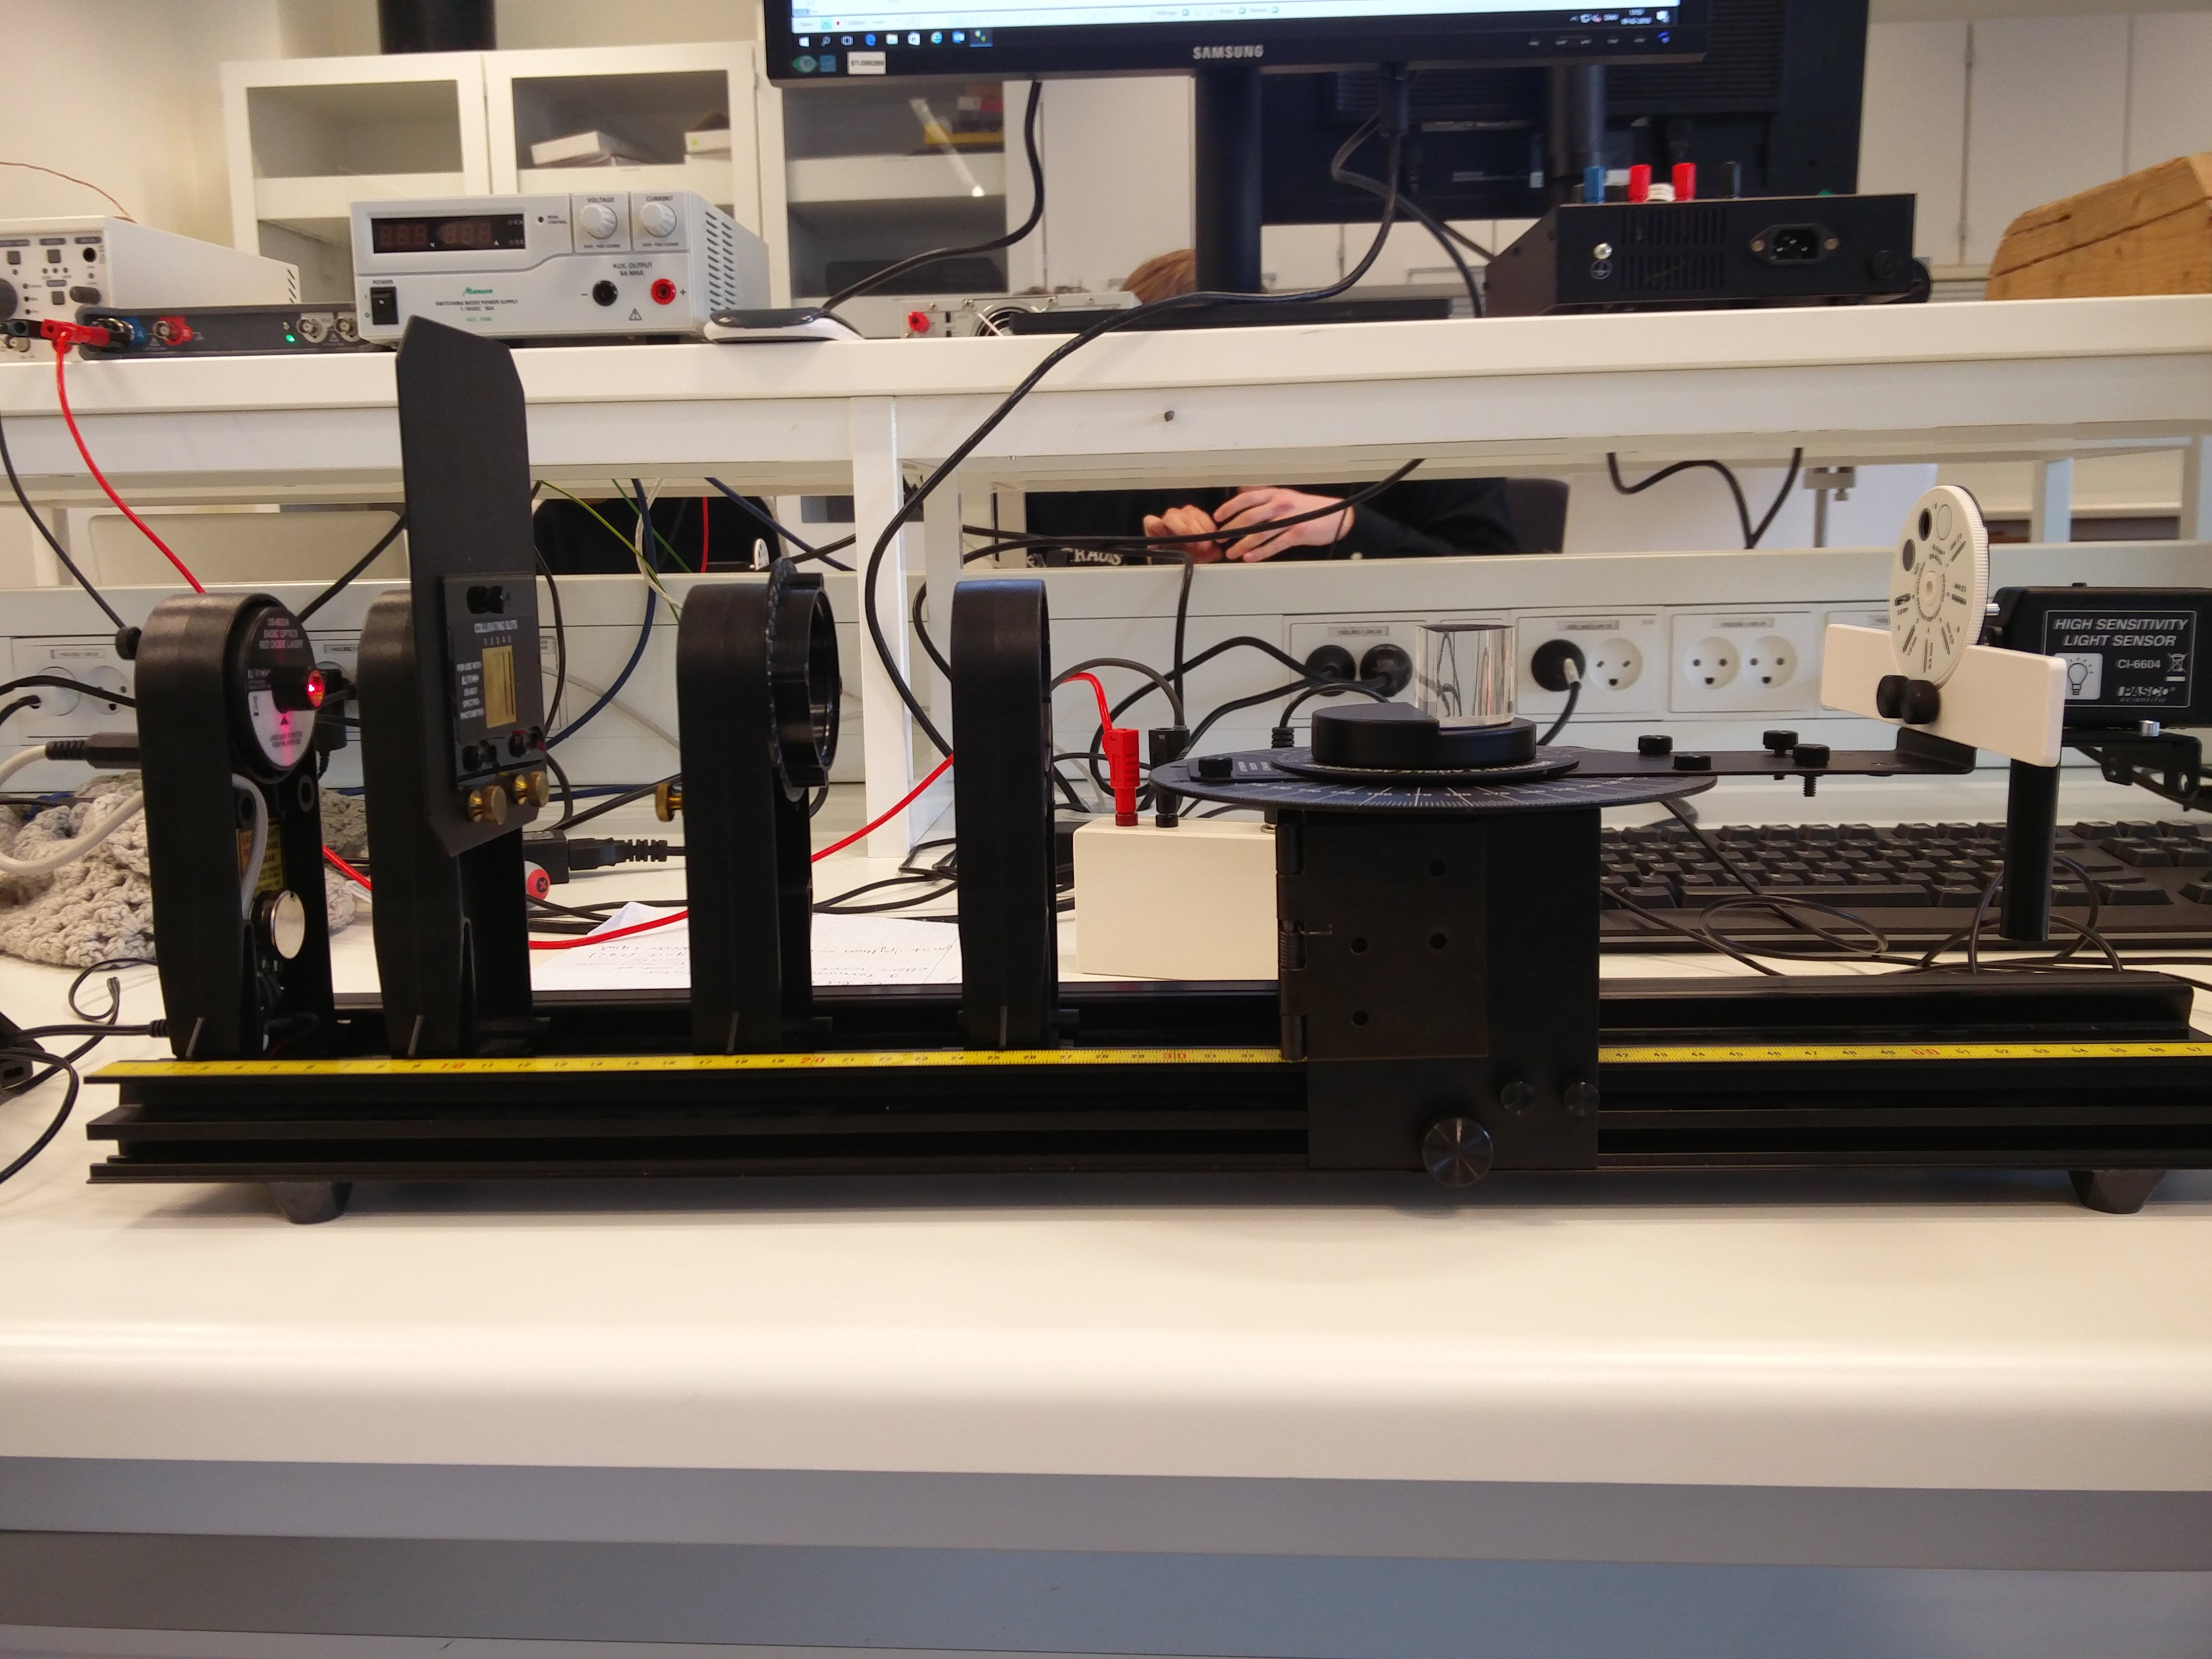
\includegraphics[trim={0 25cm 0 20cm}, clip, width=\columnwidth]{setup}
    \caption{Experimental setup. From left to right: Laser, collimating slit, polarizer, lense, glass, polarizer, photosensor. See logbook for description.}
    \label{fig:setup}
\end{figure}

